\documentclass[12pt,a4paper]{article} 
\usepackage[font={scriptsize,it}]{caption}
\usepackage{latexsym}
\usepackage{amsmath}
\usepackage{amssymb}
\usepackage{dsfont}
\usepackage{tikz}
\usepackage{listings}
\usepackage{ifthen}
\usepackage{paralist}
\usepackage{enumitem}
\usepackage{placeins}

\parskip        0mm
\oddsidemargin  0in
\evensidemargin 0in
\textwidth      6in
\topmargin      0in
\marginparwidth 30pt
\textheight     9.2in
\headheight     .1in
\headsep        .1mm

\lstset{
  basicstyle=\footnotesize\ttfamily,
  numbers=left,
  numberstyle=\tiny,
  numbersep=10pt,
  tabsize=4,
  extendedchars=true,
  breaklines=true,
  keywordstyle=\ttfamily,
  stringstyle=\ttfamily,
  showspaces=false,
  showtabs=false,
  xleftmargin=17pt,
  framexleftmargin=17pt,
  framexrightmargin=5pt,
  framexbottommargin=4pt,
  showstringspaces=false   
}
\lstloadlanguages{ 
  C , C++, ml
}

\title{VU Parallel Computing\\ 
\Large Project Report}
\author{Name: \underline{Stefan Marschner, Moritz Macke}\qquad
  Matr. number: \underline{1426962, 0327088}}
\date{Due: January 30th, 2017}


\begin{document}

\maketitle
\tableofcontents
\section{Abstract}

We present three different implementations of a parallelized Quicksort algorithm in MPI, Cilk and OpenMP. By testing the implementations on multi-core systems we aim to compare the different algorithms in terms of runtime, speedup compared to the sequential algorithm as well as efficiency (speedup per thread).

\section{Implementation - General}

For the OpenMP and Cilk implementations a similar approach was used, utilizing prefix sums to parallelize the partition step of the Quicksort algorithm. Furthermore the data is partitioned in the same way, between separation elements less than and equal from those greater than the pivot. The data size is therefore reduced only by one in the worst case, which is encountered if all elements are equal. These algorithms therefore are not suitable for data with more than a very small amount of equal elements. This issue could have easily been remedied in the simpler implementation variants but was left as is, since it was difficult to fix in the cilk2 variant, and the benchmark tests were conducted only on uniform random data in the range [0-n]. Furthermore all variants fall back onto the libc qsort function for sequentially sorting data as this was found to be significantly faster than self coded attempts. 
Choosing a fixed pivot, from the start, middle, end or the median of those three proved to behave very badly in the case of sorted sequences, therefore the median of a number of randomly chosen elements is chosen for partitioning in all implementations. 
All OpenMP and Cilk variants are generic and can be used to sort any type if provided with a suitable compare function and type size, though only (unsigned) integer and double types were tested. For simplicity reasons the MPI variant was only implemented for integers.

\section{Test System and Methology}
Tests were conducted on sequences of randomly generated positive numbers in the range [0-n], where n is the length of the sequence. The majority of tests was run only on different sizes of integer type arrays. Each test was repeated about 20 times, which turned out to be on the low side for some tests, with noise still being quite evident. However it allowed for a wider range of coverage without taking an excessive amount of time. The Cilk variants need an additional argument in the chunk size, which was fixed to n/200, always giving 200 chunks for the first partition step for the general tests. This is certainly not optimal for all sizes and processor counts and it is expected that performance could be improved by more carefully chosen numbers.\newline\newline
\textbf{OpenMP \& Cilk}\newline
The 48 core "saturn" server was made available to the students by the university. However by the time all programs were finished (and bug free) the server was hopelessly overburdened and no consistent results could be gathered. Therefore we decided to rent a server instance from Amazon EC2 for a few hours to run our tests on. This was a c4 compute optimized instance with 36 (virtualized) cores, the physical underlying machine uses \emph{Intel Xeon E5-2666 v3} processors with 10 cores per CPU. Sporadic testing during development and incomplete tests on the saturn server showed comparable scaling performance to our final results, therefore we believe this to have been a suitable substitute.
\newline\newline
\textbf{MPI}\newline
The "jupiter" server with the SLURM workload manager was used to test our MPI implementation. 

\section{OpenMP}

\subsection{Algorithm}

The OpenMP version uses a simple approach using prefix sums in a recursive implementation of Quicksort.
At the start of the Quicksort function the number of threads participating in this step is checked and, if there are more than one, the array is partitioned in parallel.
In the partition step each processor gets a chunk of the array and partitions it into a buffer of size $\frac{n}{p}$, counts the number of less than or equal elements and stores it in a shared array. Thereafter it needs to synchronize with the other processors and the exclusive prefix sum is calculated for each of the chunks, which allows each processor to write both the smaller-equal and greater parts from the buffer back into the correct section of the array.
The prefix step is currently implemented sequentially, since parallelization would not pay off with the small number of processors involved.
After the partition step is concluded all elements are on the right side of the array and the pivot is switched in between.  Since the partition work is divided into (essentially) equal sized chunks in both partition phases each processor has to do an equal amount of work in regards to comparisons, memory reads and writes. The partition step should therefore be balanced, regardless of the choice of pivot, though this does not mean the algorithm as a whole is balanced, which depends on the quality of the split.
The available processors are subsequently split into lower and upper halves, attempting to do some crude balancing according to the size of the two subsequences, and the Quicksort function is called recursively with the desired number of processors per half.
Once the number of threads taking part drops to one the algorithm switches to a Quicksort variant with sequential partition but tries to keep some parallelism by using tasks for the recursive calls. Once the array size drops below a threshold it is sorted purely sequentially.

\subsection{Analysis}
Every partition takes $\frac{n}{p} + p$ time, since both $n$ and $p$ are expected to about halve each step every spends $(\frac{n}{p})\log p + p$ time here. Assuming we are somewhat balanced each processor then takes $(\frac{n}{p})\log(\frac{n}{p})$ time to sort the data sequentially. This gives an overall time of $T_{par}$ = $O(n\log (\frac{n}{p})/p + (n\log p)/p + p)$ = $O(n\log (\frac{n}{p}) + p)$. With unlimited processors the first term tends towards 0, so $T_{\infty}$ = p, with a parallelism of $O((n\log n)/p)$. 

The total work performed by the algorithm is $p(\frac{n}{p})\log(\frac{n}{p})$ for sequential sorting, $n\log p$ for partitioning the data and $p\log p$ for pivot selection and prefix sums. Hence $W_{par}$ = $n\log(\frac{n}{p}) + n*\log p + p\log p$ = $n*\log n + p\log p$ = $O(n\log n)$ for fixed $p$, the algorithm should therefore be work optimal. It is cost optimal for $O(n) = p^2$.


\section{Cilk}
\subsection{Algorithm}
\textbf{First Variant (cilk0)}\newline
This Algorithm functions very similar to the OpenMP variant. During partitioning the data is written into a buffer array and in a second pass back into the original array. It therefore uses $O(n)$ additional space, plus $O(c)$ in each partition step, where c is the number of chunks = number of Cilk spawns. 
The main difference from the OpenMP version lies in how the Cilk system operates, as additional workers can only be spawned by function calls. Two passes are needed for partitioning between which synchronization is necessary. In each pass the work is divided with recursive calls and cilk\_spawn until it is small enough for sequential processing. The downside to this approach is that the overhead to spawn the Cilk workers is incurred twice and there is no guarantee a worker in the second pass is assigned a chunk it worked on in the first pass. It is however by far the easiest to implement and requires no additional synchronization except the one provided by Cilk. The process of spawning the Cilk tasks is also used to calculate the prefix sums required in the second pass. While the assigned chunks have equal size, generally more tasks are spawned than available processors and the balancing in detail is left to the Cilk system.
\newline\newline
\textbf{Second Variant (cilk1)}\newline
The motivation for this variant was trying to minimize the number of writes to memory and seeing if this improves performance over the first variant. It operates in the same way, using two arrays, but instead of partitioning the assigned chunk in the first pass each worker only counts the number of less than or equal elements. The prefix sum is calculated and in the second pass the data is written out to the second array, each worker knowing where to write its elements thanks to the prefix sum. 
Then the roles of the arrays are switched for the following recursive calls to Quicksort. Part of the data may end up in the secondary array after the parallel phase ends, therefore first has to be moved back to the main array, this can be combined with a partition step however so the overhead should not be too large. Overall the performance of this variant turned out to be disappointing though, as is evident from the benchmarks in Section 7.
\newline\newline
\textbf{Third Variant (cilk2)}\newline
The focus here was to minimize the memory used and attempt to sort the data in place. The only additional memory required is the one for holding the chunk information. Like in the cilk0 variant in a first pass each chunk is partitioned, counted, and used to calculate a prefix sum. The side to which smaller and bigger elements are partitioned is alternated so as to generate less and longer runs, though it is not known whether this actually has a performance impact. The essential difference lies in the second pass. First the amount of swaps necessary to finish the partitioning is calculated and then divided evenly among the tasks (as long as there is more than a minimum). Each worker then computes the two locations above and below the split point (final pivot location), to start swapping elements. Using the partial prefix sums computed in the first pass this can be accomplished in $O(\log c)$ time. This variant turned out to perform the best.
\subsection{Analysis}
The spawning of Cilk tasks and the prefix sum calculation take $\log p$ time in each step, where $p$ roughly halves every time, so $O(\log p)$ overall for each processor. The partitioning of the data itself makes up $O((\frac{n}{p})\log p)$ again, plus the sort at the end with $(\frac{n}{p})\log(\frac{n}{p})$ which gives a $T_{par}$ time of $O((n\log\frac{n}{p})/p + (n\log p)/p + \log p)$ = $O((n\log n)/p + \log p)$, with $T_{\infty}$ = $\log p$ and a parallelism of $O((n\log n)/p)$. It should be cost optimal for $O(n) = p\log p$. 

The total work performed by the algorithm is $p\log p$ for prefix sums, $\log^2 p$ for spawning the Cilk tasks, $n\log p$ for partitioning the data and $p(\frac{n}{p})\log(\frac{n}{p})$ sorting it. $W_{par}$ is then $n\log\frac{n}{p} + n\log p + p\log p + \log^2p$ = $O(n\log n + p\log p)$ = $O(n\log n)$ for fixed $p$, which makes it work optimal.

\section{Test Results - Cilk, OpenMP}
\begin{figure}[h]
	\includegraphics[width=0.9\textwidth]{img/omp_cilk_1mil.pdf}
	\caption{Runtime, efficiency and speedup results of the OpenMP/Cilk implementations for $n=10^{6}$.}
\end{figure}
\begin{figure}[h]
	\includegraphics[width=0.9\textwidth]{img/omp_cilk_10mil.pdf}
	\caption{Runtime, efficiency and speedup results of the OpenMP/Cilk implementations for $n=10^{7}$.}
\end{figure}
\begin{figure}[h]
	\includegraphics[width=0.9\textwidth]{img/omp_cilk_double_comparison_100mil.pdf}
	\caption{Speedup comparison integer vs. double for $n=10^{8}$.}
\end{figure}
\begin{figure}[h]
	\includegraphics[width=0.9\textwidth]{img/omp_cilk_speedup_10p.pdf}
	\caption{Speedup comparison with 10 processors for various data sizes $n$.}
\end{figure}
\begin{figure}[h]
	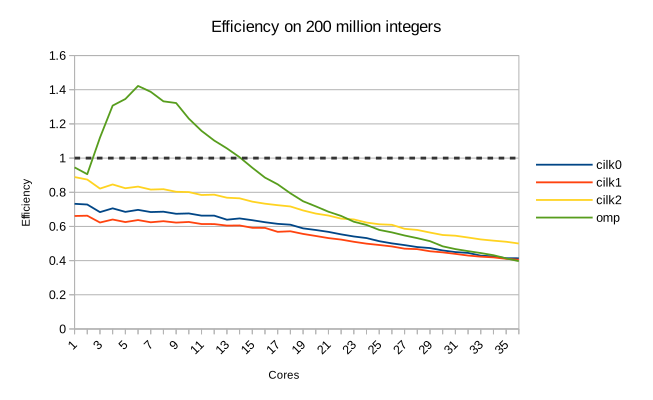
\includegraphics[width=0.9\textwidth]{img/eff_200_mil.pdf}
	\caption{Efficiency results of the OpenMP/Cilk implementations for $n=2*10^8$.}
\end{figure}

\noindent\textbf{Runtime, Speed and Efficiency}\newline
As expected, the runtime of the algorithm stagnates at about 10 threads due to the implementation overhead and hardware limitations on the test server. After this point, the results for the OpenMP implementation get noticeably worse than the Cilk counterparts (most evident from \emph{Figure 1}. This behavior of the OpenMP implementation does not seem to be accelerated by higher input size, however. In \emph{Figure 2}, the OpenMP implementation already performs much better for a higher number of threads. In our tests we found that for even bigger data sizes the OpenMP implementation would be almost as fast as the Cilk implementations. However, it is clear that something has gone wrong with the tests for the OpenMP program. With a low number of cores the speedup is super-linear, this comes not from any kind of superior algorithm. The partition part especially is actually an order of magnitude slower than standard Quicksort partition when executed sequentially. What we think happened is that more cores were recruited than requested, possibly in the phase after parallel partition other processes besides those involved in partitioning could pick up the generated tasks. What is evident in any case is that the program doesn't scale very well at all at higher number of processes.

The in-place variant Cilk2 is clearly superior to the other two and shows some nice scaling behaviour even if leveling off at the end is evident. Cilk0 performs quite well also considering it is a very simple and obvious first implementation where not much thought has been spent on optimization. The performace of Cilk1 is a disappointment, but not unexpected after local testing had already shown it to be inferior. Still there was some hope that with a high number of processes there would be a relative gain, but evidently this did not materialize.

\emph{Figure 4} shows the speedup for different data sizes with a fixed number of threads $p=10$. It is not unexpected that the speedup would be higher for bigger $n$ because the time overhead of the parallel implementation is bigger relative to the duration of the sequential algorithm for lower $n$.\newline

\noindent\textbf{Comparison - Integer and Double Input}\newline
We have also compared the speedup of the Cilk2 and OpenMP implementations for $n=10^{8}$ for integer and double arrays. The results are shown in \emph{Figure 3}. As expected, the performance is very similar, with the OpenMP implementation being about 5\% slower when doubles are used.

\FloatBarrier

\section{MPI}
\subsection{Algorithm}
The partitioning algorithm for our MPI implementation roughly works as follows:
\begin{enumerate}
	\item Divide input into (roughly) $\frac{n}{p}$ elements per process.
	\item Node 0 is arbitrarily chosen as "master", all others as "slave".
	\item At the start, all process are part of the same "set" (sets are emphasized by different colors in the graphic).
	\item Every process picks 5 elements at random and computes median, then sends it to the master.
	\item Master chooses pivots for every set of processes and sends it to them.
	\item Every process reorders their dataset using the received pivot.
	\item Depending on their rank, all processes send and receive part of a dataset to/from another process so that the lower $\frac{p}{2}$ processes only have elements smaller than the pivot and the higher $\frac{p}{2}$ processes only have elements bigger than the pivot.
	\item Every set of processes is split in half and steps 4-7 are repeated until every process is in its own set.
	\item A sequential Quicksort implementation is called in every process.
	\item Every slave sends its sorted dataset to the master, which reassembles the datasets into the full sorted array.
\end{enumerate}
However, it should be noted that the program can only be run with a number of processes that is a power of 2. However, the input size must not necessarily be a factor of the number of processes. 
\subsection{Analysis}

Time complexity of the sequential Quicksort algorithm: $T_{seq}(n)=n\cdot \log(n)$\newline
When the MPI implementation is run on $p$ processors and we assume the best case scenario where the dataset belonging to a process is always split in half, $p$ is a factor of $n$ and the communication between the processes is instant, we can assume that the complexity of the parallel algorithm is $T_{par}(n,p)=\frac{n}{p}\cdot (\log(\frac{n}{p})+\log(p))$\newline
Here, $\frac{n}{p}\cdot \log(p)$ is the complexity of the partitioning after which every process ends up with a dataset the size $\frac{n}{p}$ which is then sorted using the sequential Quicksort implementation. If we assume that we have infinite processors available we can set $p=n$ and have a time complexity of $T_{\infty}(n,p)=\log(n)$, and the \emph{parallelism} of the algorithm is therefore $\frac{T_{seq}}{T_{\infty}(n,p)}=n.$\newline
The speedup is calculated by $S_P(n) = \frac{T_{seq}}{T_{par}(n,p)} = \frac{n\cdot \log(n)}{\frac{n}{p}\cdot (\log(\frac{n}{p})+\log(p))} = p\frac{\log(n)}{\log(n)} = p$\newline
However, it should be obvious that such a speedup cannot be achieved in practice.\newline

\noindent\textbf{Drawbacks}\newline
The implementation works best for randomized input. If the array is pre-sorted, it would have a significant negative effect on the runtime of the algorithm because most of the work would be done by a single process. "Rebalancing" the datasets for a better utilization of all processes would be difficult and may not necessarily improve runtime. 
\section{Test Results - MPI}
\begin{figure}[h]
	\includegraphics[width=0.9\textwidth]{img/mpi_results.pdf}
	\caption{Runtime results of the MPI implementation for $n=10^{8}$ (left) and $n=10^{7}$ (right).}
\end{figure}
\begin{figure}[h]
	\includegraphics[width=0.9\textwidth]{img/mpi_results_sp_eff10.pdf}
	\caption{Speedup and efficiency results of the MPI implementation for $n=10^{7}$.}
\end{figure}
\begin{figure}[h]
	\includegraphics[width=0.9\textwidth]{img/mpi_results_sp_eff100.pdf}
	\caption{Speedup and efficiency results of the MPI implementation for $n=10^{8}$.}
\end{figure}


\noindent\textbf{Runtime, Speed and Efficiency}\newline
\emph{Figure 5} shows the runtime results of our implementation and \emph{Figure 6} and \emph{Figure 7} the efficiency and speedup results. Even for a high number of processes a respectable speedup can be achieved, at least until about $p=256$ where the communication overhead decreases the performance significantly. As evident from the efficiency results, the algorithm scales more poorly the higher the number of processes is. At $p=32$ and above the algorithm is obviously inefficient because the number of physical cores on the system is exceeded by the number of processes.
\newline\newline
/FloatBarrier
\textbf{Pivot Selection}\newline
As noted above, in our implementation the median of 5 random elements is sent to the master, which calculates the median of all received pivots from a set of processors and sends this new pivot back to the set of processors. We tested our implementation with $n=10^{8}$, $p=128$ and different numbers of elements randomly selected for the calculation of the pivot. The results are shown in \emph{Figure 8} We also tested the case that the pivot is always 0. This is the worst case scenario in which every element is received by processor 0 and the algorithm degenerates into sequential Quicksort with the additional overhead of the partitioning. In this case, the program runs 30\% slower than the sequential algorithm.
\begin{figure}[h]
	\includegraphics[width=0.6\textwidth]{img/mpi_pivot.pdf}
	\caption{Runtime for $n=10^{8}$ and 128 processes, different number of elements to compute pivot.}
\end{figure}
\newline\newline

\section{Conclusion}

For all our parallelized Quicksort implementations, a good speedup could be achieved. We did, however, see that the limits of parallel computing are noticeable even though the Quicksort algorithm itself is very suitable for parallelization. At 16 threads and above (and even sooner for the OpenMP implementation), the implementation overhead already makes the speedup stagnate. The MPI implementation also suffers from the same limitations, and while the speedup results look better than for Cilk/OpenMP it should be noted that a (somewhat) linear speedup for exponentially higher number of processors is not desirable in practise.

\begin{figure}[h]
	\includegraphics[width=0.8\textwidth]{img/mpi_rel_time.pdf}
	\caption{Percentage of total time spent per task by MPI master process for $n=10^{8}$.}
\end{figure}


\end{document}
